\documentclass[12pt,twoside,]{pinp}

%% Some pieces required from the pandoc template
\providecommand{\tightlist}{%
  \setlength{\itemsep}{0pt}\setlength{\parskip}{0pt}}

% Use the lineno option to display guide line numbers if required.
% Note that the use of elements such as single-column equations
% may affect the guide line number alignment.

\usepackage[T1]{fontenc}
\usepackage[utf8]{inputenc}

% pinp change: the geometry package layout settings need to be set here, not in pinp.cls
\geometry{layoutsize={0.95588\paperwidth,0.98864\paperheight},%
  layouthoffset=0.02206\paperwidth, layoutvoffset=0.00568\paperheight}

\definecolor{pinpblue}{HTML}{185FAF}  % imagecolorpicker on blue for new R logo
\definecolor{pnasbluetext}{RGB}{101,0,0} %

\usepackage{setspace} \onehalfspacing
\usepackage{booktabs}
\usepackage{longtable}
\usepackage{array}
\usepackage{multirow}
\usepackage{wrapfig}
\usepackage{float}
\usepackage{colortbl}
\usepackage{pdflscape}
\usepackage{tabu}
\usepackage{threeparttable}
\usepackage{threeparttablex}
\usepackage[normalem]{ulem}
\usepackage{makecell}
\usepackage{xcolor}

\title{Validating the perioperative thirst discomfort scale for
measuring thirst discomfort prior to procedures}

\author[]{}


\setcounter{secnumdepth}{0}

% Please give the surname of the lead author for the running footer
\leadauthor{Blinded for peer review}

% Keywords are not mandatory, but authors are strongly encouraged to provide them. If provided, please include two to five keywords, separated by the pipe symbol, e.g:
 \keywords{  fasting |  anesthesia |  thirst
discomfort |  patient-reported outcomes |  scale validation |  mokken
scale analysis  }

\begin{abstract}
\emph{Introduction:} Thirst discomfort is common because patients are
required to undergo long periods of fasting before medical and surgical
procedures. The aim of this study was to examine the validity and
reliability of the perioperative thirst discomfort scale (PTDS) for
measuring thirst discomfort before procedures. \emph{Methods:} Fasting
patients who were scheduled for an elective cardiac or interventional
radiology procedure were included in a prospective observational study.
Mokken scaling analysis was used to investigate the dimensionality and
hierarchical nature of the PTDS. PTDS scores were compared with fasting
duration to evaluate construct validity. Convergent validity was
evaluated by comparing the PTDS with global thirst discomfort and thirst
intensity ratings. \emph{Results:} Five items from the perioperative
thirst discomfort scale (PTDS-5) formed a Mokken scale with evidence of
invariant item ordering. Participants most easily endorsed the item
related to the desire to drink water through to first endorsing symptoms
related to dryness of the mouth and lips before those related to the
abnormal sensations of `thick' saliva and a `thick' tongue. Scale
reliability was adequate (rho = 0.84). There was a positive correlation
between PTDS-5 scores and the global thirst discomfort rating (tau =
0.54; 95\% CI = 0.43 to 0.63), as well as thirst intensity (tau = 0.49;
95\% CI = 0.38 to 0.59). Duration of fasting was not associated with
PTDS-5 scores. \emph{Conclusion:} The items in the PTDS-5 form a strong
Mokken scale, meaning it is a reliable and precise way to order patients
according to their thirst discomfort.
\end{abstract}

\dates{Blinded for peer review}

% initially we use doi so keep for backwards compatibility
% new name is doi_footer

\pinpfootercontents{Perioperative thirst discomfort scale}

\begin{document}

% Optional adjustment to line up main text (after abstract) of first page with line numbers, when using both lineno and twocolumn options.
% You should only change this length when you've finalised the article contents.
\verticaladjustment{-2pt}

\maketitle
\thispagestyle{firststyle}
\ifthenelse{\boolean{shortarticle}}{\ifthenelse{\boolean{singlecolumn}}{\abscontentformatted}{\abscontent}}{}

% If your first paragraph (i.e. with the \dropcap) contains a list environment (quote, quotation, theorem, definition, enumerate, itemize...), the line after the list may have some extra indentation. If this is the case, add \parshape=0 to the end of the list environment.


\hypertarget{introduction}{%
\section{Introduction}\label{introduction}}

Pre-procedure fasting is used to reduce the risk of vomiting and
aspiration pneumonia during sedation and general anaesthesia, or in case
emergency intubation is required due to unexpected cardiac arrest
\citep{hamid2014pre, osborne2002preoperative}. However, prolonged fluid
restriction causes thirst symptoms to develop (e.g., dry mouth, swollen
tongue), which can lead to great discomfort
\citep{madsen1998perioperative}. Current guidelines related to
pre-procedure fasting for elective procedures recommend a minimum
fasting period of 2 hours nil-per-os (NPO) for clear fluids
\citep{dobsonGuidelinesPracticeAnesthesia2018}. Despite these
recommendations, current practice is for patients undergoing surgical
and other medical procedures that require sedation or anesthesia to
receive standardized `nil-by-mouth' fasting instructions at a
pre-specified time interval before procedures. For example, `no eating
or drinking after midnight' is most common. It is not common for fasting
instructions to be updated even when there are significant delays in
procedure start time. As a result, fasting durations far exceed the
recommended requirement for most patients undergoing medical and
surgical procedures
\citep{de2014actual, sorita2015frequency, spitz2017impact}. For example,
in a recent study of 3641 fasting orders at a large academic institution
in the USA, it was found that the median fasting duration was 12.8
hours, averaging 2 missed meals \citep{sorita2015frequency}.

As a direct result of prolonged pre-procedure fasting, symptoms of
thirst discomfort have been reported as common and severe. In a
qualitative study where 12 participants were interviewed from a tertiary
hospital in Australia, surgical patients and patients who adhered to
prolonged fasting instructions described the discomfort from thirst
symptoms to be the worst physical effect of fasting
\citep{carey2015qualitative}. Similarly, \citep{madsen1998perioperative}
interviewed a convenience sample of 50 adult surgical patients who
reported that thirst symptoms caused more discomfort than hunger, sleep,
or anxiety related to the procedure. However, thirst and its symptoms
continue to be undervalued, under-reported and infrequently assessed by
health care providers, including the nursing team
\citep{milani2016thirst}.

Despite the relevance and value of assessing thirst-discomfort of
patients, the subjective experience of thirst presents challenges in
developing a valid and reliable tool to succinctly and accurately
measure its symptoms and level of discomfort prior to procedures. A
thirst-discomfort scale for perioperative use was developed at a
surgical centre affiliated with an accredited public hospital in Brazil
\citep{Martins_2017}. The seven-item perioperative thirst-discomfort
scale (PTDS) was developed in three stages, including face and content
validation and reliability, and based on the Consensus-based Standards
for the selection of health status Measurement Instruments (COSMIN)
checklist \citep{mokkink2010cosmin}. Inter-rater reliability was tested
through inter-observer equivalence where a pair of nurses independently,
but simultaneously administered the scale among 70 patients. Six items
on the scale had a weighted kappa coefficient of 1, while the item ``I
feel like drinking water'' was 0.97 \citep{Martins_2017}. Cronbach's
alpha was used to test the internal consistency of the scale with a
value of 0.91 \citep{Martins_2017}. It should be noted that the initial
validation of the PTDS was conducted in one specific point in the
perioperative journey (i.e.~\emph{post}-surgical patients). The
psychometric properties of the scale may be influenced by events that
occur during the surgical procedure, such as fluid loss and
administrations of medications that induce thirst, such as
glycopyrrolate. A recent large study showed that use of glycopyrrolate
was an independent risk factor for moderate to severe post-operative
thirst.\citep{lee2020prevalence} As such, validation of the scale for
measuring thirst discomfort before procedures is required.

The PTDS demonstrates strong potential for accurately assessing
thirst-discomfort more generally for peri-operative use. The aim of this
study was to examine the validity and reliability of the PTDS for
measuring thirst discomfort for patients who are fasting \emph{before}
medical procedures.

\hypertarget{methods}{%
\section{Methods}\label{methods}}

\hypertarget{study-design}{%
\subsection{Study Design}\label{study-design}}

This study used a prospective, observational design. No changes to usual
clinical practice were made for this study in regard to pre-procedure
fasting. Patients who were scheduled for a morning procedure were
typically asked to remain nil-per-os (NPO) from midnight. Patients with
afternoon procedures can have a small breakfast but must remain NPO from
6:00am on the day of the procedure. Ethical approval for this study
(Ethical Committee N° 19-5585) was provided by the University Health
Network Research Ethics Board, Toronto, Canada on October 31 2019.

\hypertarget{participants}{%
\subsection{Participants}\label{participants}}

Adult patients who were fasted and scheduled for an elective procedure
in the Cardiac Catheterization Laboratories or in Interventional
Radiology at an academic teaching hospital in Canada were included.

\hypertarget{exclusion-criteria}{%
\subsubsection{Exclusion criteria}\label{exclusion-criteria}}

Patients were not eligible for the study if they were under 16 years of
age, scheduled for an emergency procedure, unable to understand or speak
English (unless a translator was available) or if the nurse in
pre-procedure bay considered that there was insufficient time prior to
anticipated commencement of the procedure for participation in the
study.

\hypertarget{data-collection}{%
\subsection{Data collection}\label{data-collection}}

A Research Assistant administered a brief questionnaire prior to
procedures. It comprised the following components:

\begin{itemize}
\tightlist
\item
  the Perioperative Thirst Discomfort Scale (7 items);
\item
  a one-item global thirst discomfort rating;
\item
  a one-item thirst intensity rating;
\item
  an item to determine if the participant is currently on oxygen
  therapy;
\item
  an item to evaluate the presence of pain;
\item
  the time the patient last had any clear fluids;
\item
  the time the patient last had any food;
\item
  age, sex of patient and type of procedure to be performed.
\end{itemize}

\hypertarget{measures}{%
\subsubsection{Measures}\label{measures}}

The seven-item Perioperative Thirst Discomfort Scale (PTDS-7) is a
7-item self-reported, composite score evaluating the severity of dry
mouth, lips, and throat, thick tongue and saliva, a bad taste in the
mouth, and a desire to drink water.\citep{Martins_2017} The total score
can range from 0 to 14, with 14 representing the ``most extreme''
intensity of discomfort related to perioperative
thirst.\citep{Martins_2017}

Participants used a global thirst discomfort score to rate their overall
level of thirst discomfort on a rating scale with scores ranging from
``extreme thirst discomfort'' to ``extreme comfort''. Intensity of their
thirst was rated on a scale ranging from 0 to 10, where 0 represents
``No thirst'' and 10 represents ``Most intense thirst''. The experience
of pain may influence the participant's perception of
thirst.\citep{Pierotti_2018} Participants were asked to rate their
current level of pain on a scale of 0 to 10, where 0 represents ``no
pain'' and 10 represents that their pain as
``unimaginable/unspeakable''. The use of oxygen therapy (e.g., via nasal
prongs) may contribute to the experience of thirst symptoms (e.g., dry
mouth, dry throat).\citep{conchon2015perioperative} The research
assistant recorded ``yes'' or ``no'' as to whether the participant was
currently receiving oxygen therapy at the time the questionnaire was
administered.

\hypertarget{statistical-analysis}{%
\subsection{Statistical analysis}\label{statistical-analysis}}

Mokken scaling is a method for establishing if items in a scale conform
to a cumulative, hierarchical structure \citep{perng2012construct}. When
an instrument contains hierarchically ordered items, the items can be
ordered from those indicating mild to severe symptoms. An intentionally
simple example of a hierarchical scale is a set of items enquiring about
height that increases in increments of 10cm from 100cm to 200cm. In this
example, taller people would endorse more items than those who were
shorter \citep{watson2008hierarchy}.

To determine if items conform to a hierarchical structure, Mokken
scaling analyses properties of individual items as described by the item
characteristic curve. Item characteristic curves show the association
between the score on an item to the level of the latent trait being
measured. Mokken scaling makes only the assumption of monotone
homogeneity about the association between the score on an item and the
level of the latent trait. This means that as the trait increases, so
does the item score. ``Difficulty'', is a term used in Mokken Scale
Analysis to refer to the extent to which items are endorsed by
respondents. Items at the upper end of the range of the latent trait are
characterized as being more difficult. Items in a Mokken Scale are
arranged along the latent trait in terms of their difficulty. The
properties of items can be measured using the scalability coefficient,
\emph{H} (Loevinger's coefficient). \emph{H} measures the extent to
which items are arranged as expected by their mean values along the
latent trait. \emph{H} \textgreater{} 0.3 is the minimum acceptable
value, with values \textgreater{} 0.4 indicating a moderate scale and
\textgreater{} 0.5 indicates a strong scale.

Invariant item ordering, where the order of items along the latent trait
is the same for all respondents at all levels of the latent trait, is a
desirable property of a Mokken Scale. It can be assessed mathematically
to look for significant violations of this property. The accuracy of the
invariant item ordering can also be assessed by calculating the
\emph{H\textsubscript{TRANS}} (\textbf{H\textsubscript{T}}) coefficient.
Values of \textbf{H\textsubscript{T}} exceeding 0.3 indicates acceptable
accuracy of invariant item ordering.

Mokken scale analysis was conducted in this study to explore whether
there were hierarchical properties in participant ratings of thirst
discomfort and to explore the dimensions of the PTDS. Mokken scale
analysis proceeded by first checking the PTDS-7 scalability
coefficients. If \textbf{H\textsubscript{i}} was below 0.3 or if the
lower limit of the 95\% CI (confidence interval) for
\emph{H\textsubscript{i}} was below 0.3, the item was to be excluded.
Then, scale partitioning was carried out to explore the dimensions of
the PTDS through increasing c (lower bound c defines the minimum value
of coefficients \textbf{H\textsubscript{i}} in the Mokken scale by 0.05
increments) \citep{molenaar2000mps5}. Monotone homogeneity and invariant
item ordering were investigated at the whole scale level, as no
sub-scales were identified. To assess for violations of invariant item
ordering, crit values \textless40 were considered
acceptable.\citep{molenaar2000mps5} Provided invariant item ordering
holds for a set of items, the coefficient \textbf{H\textsubscript{T}}
expresses the accuracy of the ordering, with values below 0.3 being
unacceptable and above 0.4 indicating moderate invariant item
ordering.\citep{Ligtvoet_2010} The coefficient score (rho), which is
similar to Cronbach's alpha, was used to assess reliability of the
scale.

Construct validity was evaluated by using correlations to identify
associations between scores on the PTDS and fasting duration. To
investigate construct validity we hypothesized that higher scores on the
PTDS would be associated with greater fasting duration. Convergent
validity was assessed by using Kendall's \emph{tau} to compare the PTDS
score with the global thirst discomfort score. Convergent validity was
assessed by using the Spearman's rank correlation to compare the PTDS
with the thirst intensity rating and pain scale rating.

The R statistical program was used to conduct all analyses
\citep{rcore2020}. All data and R code, along with instructions for how
to completely reproduce results of the analyses, is available
\href{https://github.com/awconway/ptds}{here}. A formal sample size
calculation was not conducted.

\hypertarget{results}{%
\section{Results}\label{results}}

From November 2019 to March 2020, we screened 203 patients for inclusion
in the study. A total of 198 were eligible and 194 participated. One
participant did not complete 1 of the PTDS-7 items and was excluded from
the analysis. A summary of participant characteristics is displayed in
Table \ref{tab:tab1pdf}. The median age was 62 (IQR 48 - 72) and 58\%
(n=111) were female. 43\% of patients were scheduled to have their
procedure in the cardiac catheterization laboratory. A biopsy was the
most common interventional radiology procedure (n=62; 32\%), but a wide
range of other procedures were included. The mean duration of fasting
from food and non-clear fluids was 12.7 (SD 3.8) hours and clear fluids
was 9 (SD 4.5) hours.

\begin{table}

\caption{\label{tab:tab1pdf}Participant characteristics}
\centering
\begin{tabular}[t]{ll}
\toprule
Characteristic & N = 193\\
\midrule
Age & 62 (48, 72)\\
Gender & \\
\hspace{1em}Male & 111 (58\%)\\
\hspace{1em}Female & 80 (42\%)\\
\hspace{1em}Prefer not to say & 1 (0.5\%)\\
\addlinespace
Procedure & \\
\hspace{1em}Angiogram or Percutaneous Coronary Intervention (PCI) & 58 (30\%)\\
\hspace{1em}Cardiac Implantable Electronic Device (CIED) & 15 (7.8\%)\\
\hspace{1em}Electrophysiology Study (EPS) & 5 (2.6\%)\\
\hspace{1em}Structural heart intervention & 5 (2.6\%)\\
\addlinespace
\hspace{1em}Vascular angiography or intervention & 17 (8.9\%)\\
\hspace{1em}Biopsy & 62 (32\%)\\
\hspace{1em}Port-a-cath & 4 (2.1\%)\\
\hspace{1em}Radiofrequency ablation of a tumour (RFA) & 9 (4.7\%)\\
\hspace{1em}Vascular embolization (e.g., renal) & 1 (0.5\%)\\
\addlinespace
\hspace{1em}Other procedure & 16 (8.3\%)\\
Time since last clear fluids (hours) & 9.5 (5.0, 13.0)\\
Time since last food (hours) & 13.0 (11.0, 15.0)\\
\bottomrule
\multicolumn{2}{l}{\textsuperscript{1} Statistics presented: median (IQR); n (\%)}\\
\end{tabular}
\end{table}

\hypertarget{mokken-scale-analysis}{%
\subsection{Mokken scale analysis}\label{mokken-scale-analysis}}

No items required removal from the PTDS-7 based on the condition that
scalability coefficients (\emph{H\textsubscript{i}} and lower bound of
95\% CI) should be over 0.3. We used a lower bound for \emph{c},
starting from 0.05 and increasing to 0.80 in 0.05 increments, to explore
the dimensionality of the PTDS-7. From 0.05 to 0.45, all of the items
formed a single scale. The item, `\emph{I have a bad taste in my
mouth}', was excluded by selecting the remaining items which showed
uni-dimensionality at a threshold level of .50. The 6 remaining items
(PTDS-6) were further examined for the criteria of a Mokken scale and
item invariant ordering. The PTDS-6 item set had a homogeneity value
\emph{H(se)} of 0.599, which indicated a strong Mokken scale. No items
were removed based on the criteria that there should be no significant
violations of the assumption of monotonicity.

\hypertarget{invariant-item-ordering}{%
\subsubsection{Invariant item ordering}\label{invariant-item-ordering}}

Analysis of invariant item ordering for the PTDS-6 revealed violations
for the dry throat/dry lips item pair. Although there were no
\emph{significant} intersections between items, due to the intersection
between the dry throat and dry lips items, crit values were above 40.
For this reason, we excluded one of these items (dry throat), and
re-assessed the remaining 5 items for the assumptions of a Mokken scale.
With the dry throat item removed, none of the items violated the
assumption of invariant item ordering.

\hypertarget{accuracy-and-reliability}{%
\subsubsection{Accuracy and
reliability}\label{accuracy-and-reliability}}

The accuracy of the item ordering was found to be acceptable with a
\emph{H\textsubscript{T}} coefficient of 0.397. Scale reliability was
adequate with a coefficient score (Rho) of 0.84.

\hypertarget{item-difficulty-hierarchy}{%
\subsubsection{Item difficulty
hierarchy}\label{item-difficulty-hierarchy}}

The item difficult hierarchy for the PTDS-5 is presented in Table
\ref{tab:hierarchytabpdf}. The most highly endorsed symptom (i.e.~the
least severe symptom of thirst discomfort in the PTDS-5) was being
bothered by a desire to drink water. The least endorsed symptom
(i.e.~the most severe symptom of thirst discomfort in the PTDS-5) was
being bothered by the perception of a `thick tongue'. The items in the
PTDS-5 form a strong Mokken scale (H\textsubscript{s} = 0.605).

\begin{table}

\caption{\label{tab:hierarchytabpdf}Item hierarchy of the PTDS-5}
\centering
\begin{tabular}[t]{lrrr}
\toprule
item & mean & Hi & se\\
\midrule
I want to drink water & 1.10 & 0.56 & 0.054\\
My mouth is dry & 0.80 & 0.62 & 0.044\\
My lips are dry & 0.69 & 0.63 & 0.041\\
My saliva is thick & 0.51 & 0.57 & 0.050\\
My tongue is thick & 0.43 & 0.65 & 0.042\\
\bottomrule
\end{tabular}
\end{table}

\hypertarget{construct-and-convergent-validity}{%
\subsection{Construct and convergent
validity}\label{construct-and-convergent-validity}}

The distribution of PTDS-5 scores in the sample was right-skewed, with a
median score of 3 (IQR 1, 6). (Figure \ref{fig:distributionpdf}). As
shown in Figure \ref{fig:globalthirst}, there was a positive correlation
between PTDS-5 scores and the global thirst discomfort rating
(\emph{tau} = 0.54; 95\% CI = 0.43 to 0.63; 0). The correlation between
PTDS-5 scores and thirst intensity was also high (\emph{tau} = 0.49;
95\% CI = 0.38 to 0.59). Likewise, the correlation between pain and
PTDS-5 scores was not significant (Spearman's rho = 0.07; 95\% CI =
-0.07 to 0.21).

\begin{figure}

{\centering 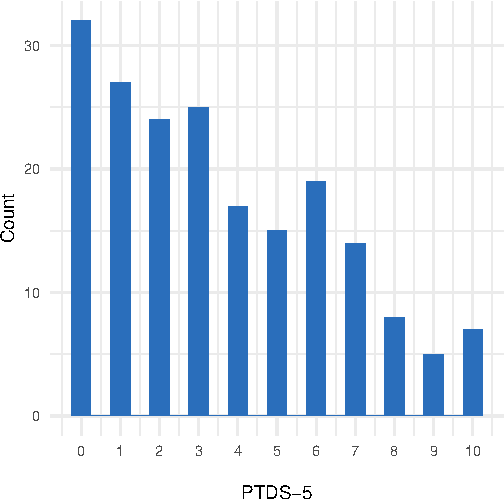
\includegraphics[width=252px]{distributionpdf-1}

}

\caption{Distribution of PTDS-5 scores (higher scores indicate worse thirst discomfort)}\label{fig:distributionpdf}
\end{figure}

\begin{figure}

{\centering 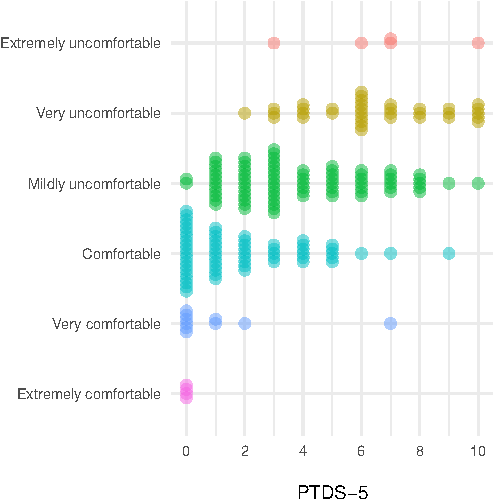
\includegraphics[width=252px]{globalthirst-1}

}

\caption{Association between PTDS-5 and global thirst rating}\label{fig:globalthirst}
\end{figure}

The associations between PTDS-5 scores with food and fluid duration are
displayed in Figure \ref{fig:fasting}. Longer duration of fasting was
not linearly associated with PTDS-5 scores for fluids (Spearman's rho =
0.1; 95\% CI = -0.05 to 0.23) or food (Spearman's rho = 0.13; 95\% CI =
-0.01 to 0.27).

\begin{figure}

{\centering 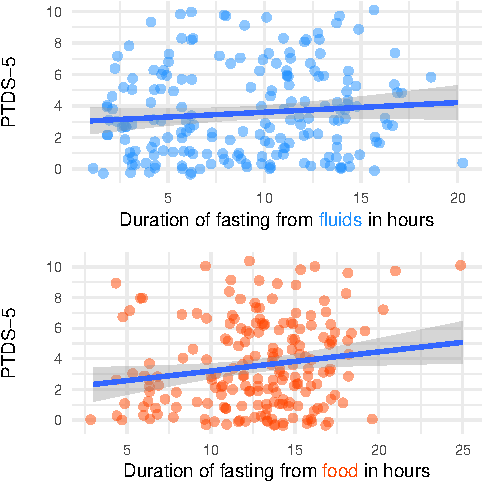
\includegraphics[width=252px]{fasting-1}

}

\caption{Association between PTDS-5 and duration of fasting}\label{fig:fasting}
\end{figure}

\hypertarget{discussion}{%
\section{Discussion}\label{discussion}}

Results indicate that the PTDS-5 is a reliable and precise way to order
patients according to their thirst discomfort in the
\emph{pre-procedure} period. In addition, an acceptable accuracy for
invariant item ordering was identified, meaning patients are likely to
rank the PTDS-5 symptoms of thirst discomfort in the same way. As such,
the item difficulty hierarchy, presented in Table
\ref{tab:hierarchytabpdf}, can be used as a guide to easily determine
which patients are experiencing worse thirst discomfort. The
hierarchical pattern of responses to items in the Mokken scale is
interpretable in terms of respondents more easily endorsing items
related to a general desire to drink water through to first endorsing
more specific symptoms related to dryness of the mouth and lips prior to
endorsing discomfort associated with the sensations of `thick' saliva
and `thick' tongue. In more practical terms, a patient who reports feeling bothered by a sensation of thick saliva could be interpreted as experiencing worse thirst discomfort than a patient who did not endorse any of the items lower down on the item difficulty hierarchy (i.e.~`my lips are dry' and `my mouth is dry').

The original (7-item) perioperative thirst-discomfort scale has
previously been used to determine the relationship between thirst
intensity and thirst-discomfort in the immediate postoperative period
during anesthesia recovery.\citep{Pierotti_2018} In a non-probabilistic
sample of 203 adult participants in post-operative recovery following
elective, urgent and emergency surgeries, the investigators found no
association between fasting duration, or patient age, and the intensity
of thirst and degree of discomfort \citep{Pierotti_2018}. However, the
mean fasting duration among participants was uniformly high (mean 16.2
{[}SD 8.7{]} hours), which may have prevented the researchers from
discerning a correlation between fasting duration. Even in the subgroup
of participant who reported 8 hours of fasting, all reported thirst
\citep{aroni2012assessment, Pierotti_2018}.

It should be noted that an investigation of the dimensionality of the
7-item PTDS had not been performed prior to our study. A uni-dimensional
solution was identified in our analysis. This should be expected
considering the small number of items that were evaluated.

We did not observe an association between PTDS-5 and fasting duration
for either food or fluids. This would suggest that it is important to
assess thirst discomfort periodically, regardless of the duration of
fasting. If thirst discomfort is present, and fasting is still
indicated, interventions to alleviate symptoms should be implemented.
There is a lack of evidence regarding the efficacy of interventions to
alleviate perioperative thirst discomfort. However, recent randomized
controlled trials have identified clinically relevant reductions in
thirst discomfort with menthol chewing gum and 30mL menthol popsicles
\citep{garcia2019, nascimento2020}. One additional potential course of
action could be to rearrange the order of procedures on a schedule based
on results of periodic thirst discomfort assessments using the PTDS. For
example, circumstance may arise where a patient who reports severe
thirst discomfort is scheduled to have their procedure later in the day
than a patient who is not currently bothered by thirst symptoms.
Reordering the procedure schedule would reduce the duration of fasting
for the patient who is bothered by symptoms of thirst. Further research
would be required to confirm the effectiveness of this strategy in
practice on overall patient satisfaction.

\hypertarget{limitations}{%
\subsection{Limitations}\label{limitations}}

Selection bias should be considered because a convenience sample was
used for this study. Also, it is uncertain if similar results would be
obtained for patients who are fasted prior to undergoing procedures in
other settings. Only one patient was excluded from the analysis due to
missing data, so it is unlikely attrition bias would have exerted a
major influence on the results. Further research is required to evaluate
the minimal detectable difference for the PTDS-5 as well as the minimal
clinically important difference prior to use of this scale as an outcome
measure in research. The potential that the sample size was insufficient
for Mokken scale analysis should be considered. A recent study
empirically evaluated the sample size required for a scale and found
that a minimum of 250 participants would be required to establish
scalability of the whole scale.\citep{watson2018} It was unclear,
however, if this minimum threshold would apply to other scales.

\hypertarget{conclusion}{%
\subsection{Conclusion}\label{conclusion}}

The items in the PTDS-5 may provide a reliable and precise way to order
patients according to their thirst discomfort. Nurses may use this scale
to assess the severity of thirst discomfort in patients who are fasted
prior to procedures and initiate interventions according to individual
needs. The PTDS-5 with the rating scale is presented in Table
\ref{tab:tabptds}.

\begin{table}

\caption{\label{tab:tabptds}5-item perioperative thirst discomfort scale (PTDS-5)}
\centering
\begin{tabular}[t]{lrrr}
\toprule
How bothered are you by the following? & Not at all & Slightly & Extremely\\
\midrule
I want to drink water & 0 & 1 & 2\\
My mouth is dry & 0 & 1 & 2\\
My lips is dry & 0 & 1 & 2\\
My saliva is thick & 0 & 1 & 2\\
My tongue is thick & 0 & 1 & 2\\
\bottomrule
\end{tabular}
\end{table}

%\showmatmethods

\pnasbreak

\bibliography{references.bib}
\bibliographystyle{jss}



\end{document}
